\documentclass[1p]{elsarticle_modified}
%\bibliographystyle{elsarticle-num}

%\usepackage[colorlinks]{hyperref}
%\usepackage{abbrmath_seonhwa} %\Abb, \Ascr, \Acal ,\Abf, \Afrak
\usepackage{amsfonts}
\usepackage{amssymb}
\usepackage{amsmath}
\usepackage{amsthm}
\usepackage{scalefnt}
\usepackage{amsbsy}
\usepackage{kotex}
\usepackage{caption}
\usepackage{subfig}
\usepackage{color}
\usepackage{graphicx}
\usepackage{xcolor} %% white, black, red, green, blue, cyan, magenta, yellow
\usepackage{float}
\usepackage{setspace}
\usepackage{hyperref}

\usepackage{tikz}
\usetikzlibrary{arrows}

\usepackage{multirow}
\usepackage{array} % fixed length table
\usepackage{hhline}

%%%%%%%%%%%%%%%%%%%%%
\makeatletter
\renewcommand*\env@matrix[1][\arraystretch]{%
	\edef\arraystretch{#1}%
	\hskip -\arraycolsep
	\let\@ifnextchar\new@ifnextchar
	\array{*\c@MaxMatrixCols c}}
\makeatother %https://tex.stackexchange.com/questions/14071/how-can-i-increase-the-line-spacing-in-a-matrix
%%%%%%%%%%%%%%%

\usepackage[normalem]{ulem}

\newcommand{\msout}[1]{\ifmmode\text{\sout{\ensuremath{#1}}}\else\sout{#1}\fi}
%SOURCE: \msout is \stkout macro in https://tex.stackexchange.com/questions/20609/strikeout-in-math-mode

\newcommand{\cancel}[1]{
	\ifmmode
	{\color{red}\msout{#1}}
	\else
	{\color{red}\sout{#1}}
	\fi
}

\newcommand{\add}[1]{
	{\color{blue}\uwave{#1}}
}

\newcommand{\replace}[2]{
	\ifmmode
	{\color{red}\msout{#1}}{\color{blue}\uwave{#2}}
	\else
	{\color{red}\sout{#1}}{\color{blue}\uwave{#2}}
	\fi
}

\newcommand{\Sol}{\mathcal{S}} %segment
\newcommand{\D}{D} %diagram
\newcommand{\A}{\mathcal{A}} %arc


%%%%%%%%%%%%%%%%%%%%%%%%%%%%%5 test

\def\sl{\operatorname{\textup{SL}}(2,\Cbb)}
\def\psl{\operatorname{\textup{PSL}}(2,\Cbb)}
\def\quan{\mkern 1mu \triangleright \mkern 1mu}

\theoremstyle{definition}
\newtheorem{thm}{Theorem}[section]
\newtheorem{prop}[thm]{Proposition}
\newtheorem{lem}[thm]{Lemma}
\newtheorem{ques}[thm]{Question}
\newtheorem{cor}[thm]{Corollary}
\newtheorem{defn}[thm]{Definition}
\newtheorem{exam}[thm]{Example}
\newtheorem{rmk}[thm]{Remark}
\newtheorem{alg}[thm]{Algorithm}

\newcommand{\I}{\sqrt{-1}}
\begin{document}

%\begin{frontmatter}
%
%\title{Boundary parabolic representations of knots up to 8 crossings}
%
%%% Group authors per affiliation:
%\author{Yunhi Cho} 
%\address{Department of Mathematics, University of Seoul, Seoul, Korea}
%\ead{yhcho@uos.ac.kr}
%
%
%\author{Seonhwa Kim} %\fnref{s_kim}}
%\address{Center for Geometry and Physics, Institute for Basic Science, Pohang, 37673, Korea}
%\ead{ryeona17@ibs.re.kr}
%
%\author{Hyuk Kim}
%\address{Department of Mathematical Sciences, Seoul National University, Seoul 08826, Korea}
%\ead{hyukkim@snu.ac.kr}
%
%\author{Seokbeom Yoon}
%\address{Department of Mathematical Sciences, Seoul National University, Seoul, 08826,  Korea}
%\ead{sbyoon15@snu.ac.kr}
%
%\begin{abstract}
%We find all boundary parabolic representation of knots up to 8 crossings.
%
%\end{abstract}
%\begin{keyword}
%    \MSC[2010] 57M25 
%\end{keyword}
%
%\end{frontmatter}

%\linenumbers
%\tableofcontents
%
\newcommand\colored[1]{\textcolor{white}{\rule[-0.35ex]{0.8em}{1.4ex}}\kern-0.8em\color{red} #1}%
%\newcommand\colored[1]{\textcolor{white}{ #1}\kern-2.17ex	\textcolor{white}{ #1}\kern-1.81ex	\textcolor{white}{ #1}\kern-2.15ex\color{red}#1	}

{\Large $\underline{11a_{324}~(K11a_{324})}$}

\setlength{\tabcolsep}{10pt}
\renewcommand{\arraystretch}{1.6}
\vspace{1cm}\begin{tabular}{m{100pt}>{\centering\arraybackslash}m{274pt}}
\multirow{5}{120pt}{
	\centering
	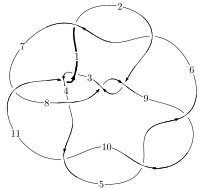
\includegraphics[width=112pt]{../../../GIT/diagram.site/Diagrams/png/573_11a_324.png}\\
\ \ \ A knot diagram\footnotemark}&
\allowdisplaybreaks
\textbf{Linearized knot diagam} \\
\cline{2-2}
 &
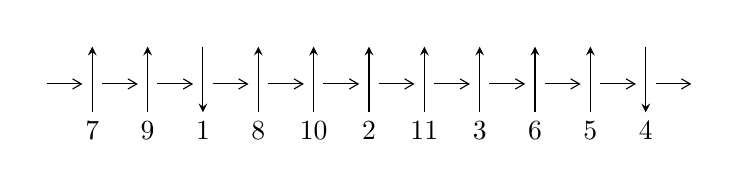
\begin{tikzpicture}[x=20pt, y=17pt]
	% nodes
	\node (C0) at (0, 0) {};
	\node (C1) at (1, 0) {};
	\node (C1U) at (1, +1) {};
	\node (C1D) at (1, -1) {7};

	\node (C2) at (2, 0) {};
	\node (C2U) at (2, +1) {};
	\node (C2D) at (2, -1) {9};

	\node (C3) at (3, 0) {};
	\node (C3U) at (3, +1) {};
	\node (C3D) at (3, -1) {1};

	\node (C4) at (4, 0) {};
	\node (C4U) at (4, +1) {};
	\node (C4D) at (4, -1) {8};

	\node (C5) at (5, 0) {};
	\node (C5U) at (5, +1) {};
	\node (C5D) at (5, -1) {10};

	\node (C6) at (6, 0) {};
	\node (C6U) at (6, +1) {};
	\node (C6D) at (6, -1) {2};

	\node (C7) at (7, 0) {};
	\node (C7U) at (7, +1) {};
	\node (C7D) at (7, -1) {11};

	\node (C8) at (8, 0) {};
	\node (C8U) at (8, +1) {};
	\node (C8D) at (8, -1) {3};

	\node (C9) at (9, 0) {};
	\node (C9U) at (9, +1) {};
	\node (C9D) at (9, -1) {6};

	\node (C10) at (10, 0) {};
	\node (C10U) at (10, +1) {};
	\node (C10D) at (10, -1) {5};

	\node (C11) at (11, 0) {};
	\node (C11U) at (11, +1) {};
	\node (C11D) at (11, -1) {4};
	\node (C12) at (12, 0) {};

	% arrows
	\draw[->,>={angle 60}]
	(C0) edge (C1) (C1) edge (C2) (C2) edge (C3) (C3) edge (C4) (C4) edge (C5) (C5) edge (C6) (C6) edge (C7) (C7) edge (C8) (C8) edge (C9) (C9) edge (C10) (C10) edge (C11) (C11) edge (C12) ;	\draw[->,>=stealth]
	(C1D) edge (C1U) (C2D) edge (C2U) (C3U) edge (C3D) (C4D) edge (C4U) (C5D) edge (C5U) (C6D) edge (C6U) (C7D) edge (C7U) (C8D) edge (C8U) (C9D) edge (C9U) (C10D) edge (C10U) (C11U) edge (C11D) ;
	\end{tikzpicture} \\
\hhline{~~} \\& 
\textbf{Solving Sequence} \\ \cline{2-2} 
 &
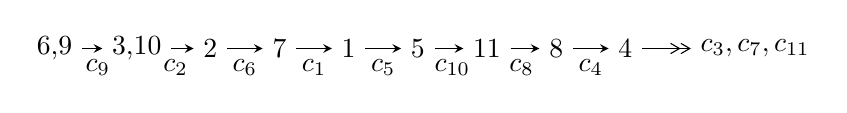
\begin{tikzpicture}[x=25pt, y=7pt]
	% node
	\node (A0) at (-1/8, 0) {6,9};
	\node (A1) at (17/16, 0) {3,10};
	\node (A2) at (17/8, 0) {2};
	\node (A3) at (25/8, 0) {7};
	\node (A4) at (33/8, 0) {1};
	\node (A5) at (41/8, 0) {5};
	\node (A6) at (49/8, 0) {11};
	\node (A7) at (57/8, 0) {8};
	\node (A8) at (65/8, 0) {4};
	\node (C1) at (1/2, -1) {$c_{9}$};
	\node (C2) at (13/8, -1) {$c_{2}$};
	\node (C3) at (21/8, -1) {$c_{6}$};
	\node (C4) at (29/8, -1) {$c_{1}$};
	\node (C5) at (37/8, -1) {$c_{5}$};
	\node (C6) at (45/8, -1) {$c_{10}$};
	\node (C7) at (53/8, -1) {$c_{8}$};
	\node (C8) at (61/8, -1) {$c_{4}$};
	\node (A9) at (10, 0) {$c_{3},c_{7},c_{11}$};

	% edge
	\draw[->,>=stealth]	
	(A0) edge (A1) (A1) edge (A2) (A2) edge (A3) (A3) edge (A4) (A4) edge (A5) (A5) edge (A6) (A6) edge (A7) (A7) edge (A8) ;
	\draw[->>,>={angle 60}]	
	(A8) edge (A9);
\end{tikzpicture} \\ 

\end{tabular} \\

\footnotetext{
The image of knot diagram is generated by the software ``\textbf{Draw programme}" developed by Andrew Bartholomew(\url{http://www.layer8.co.uk/maths/draw/index.htm\#Running-draw}), where we modified some parts for our purpose(\url{https://github.com/CATsTAILs/LinksPainter}).
}\phantom \\ \newline 
\centering \textbf{Ideals for irreducible components\footnotemark of $X_{\text{par}}$} 
 
\begin{align*}
I^u_{1}&=\langle 
5 u^{20}-59 u^{19}+\cdots+16 b+720,\;-35 u^{20}+367 u^{19}+\cdots+32 a-1520,\;u^{21}-11 u^{20}+\cdots+368 u-32\rangle \\
I^u_{2}&=\langle 
-6.48197\times10^{26} a^{9} u^{3}-2.24957\times10^{27} a^{8} u^{3}+\cdots+6.21716\times10^{28} a+6.82138\times10^{28},\\
\phantom{I^u_{2}}&\phantom{= \langle  }2 a^9 u^3-3 a^8 u^3+\cdots-72 a+3,\;u^4+u^3+3 u^2+2 u+1\rangle \\
I^u_{3}&=\langle 
- u^6-4 u^4+u^3-4 u^2+b+u,\;- u^6- u^5-4 u^4-3 u^3-3 u^2+a-3 u+1,\\
\phantom{I^u_{3}}&\phantom{= \langle  }u^{12}+8 u^{10}- u^9+24 u^8-4 u^7+32 u^6-4 u^5+16 u^4+u^2+1\rangle \\
\\
\end{align*}
\raggedright * 3 irreducible components of $\dim_{\mathbb{C}}=0$, with total 73 representations.\\
\footnotetext{All coefficients of polynomials are rational numbers. But the coefficients are sometimes approximated in decimal forms when there is not enough margin.}
\newpage
\renewcommand{\arraystretch}{1}
\centering \section*{I. $I^u_{1}= \langle 5 u^{20}-59 u^{19}+\cdots+16 b+720,\;-35 u^{20}+367 u^{19}+\cdots+32 a-1520,\;u^{21}-11 u^{20}+\cdots+368 u-32 \rangle$}
\flushleft \textbf{(i) Arc colorings}\\
\begin{tabular}{m{7pt} m{180pt} m{7pt} m{180pt} }
\flushright $a_{6}=$&$\begin{pmatrix}0\\u\end{pmatrix}$ \\
\flushright $a_{9}=$&$\begin{pmatrix}1\\0\end{pmatrix}$ \\
\flushright $a_{3}=$&$\begin{pmatrix}1.09375 u^{20}-11.4688 u^{19}+\cdots-488.500 u+47.5000\\-\frac{5}{16} u^{20}+\frac{59}{16} u^{19}+\cdots+425 u-45\end{pmatrix}$ \\
\flushright $a_{10}=$&$\begin{pmatrix}1\\- u^2\end{pmatrix}$ \\
\flushright $a_{2}=$&$\begin{pmatrix}1.40625 u^{20}-15.1563 u^{19}+\cdots-913.500 u+92.5000\\-\frac{5}{16} u^{20}+\frac{59}{16} u^{19}+\cdots+425 u-45\end{pmatrix}$ \\
\flushright $a_{7}=$&$\begin{pmatrix}-\frac{5}{4} u^{20}+\frac{51}{4} u^{19}+\cdots+360 u-\frac{63}{2}\\u^{20}-\frac{21}{2} u^{19}+\cdots-\frac{855}{2} u+40\end{pmatrix}$ \\
\flushright $a_{1}=$&$\begin{pmatrix}\frac{27}{16} u^{20}-\frac{139}{8} u^{19}+\cdots-939 u+95\\-\frac{23}{16} u^{20}+\frac{231}{16} u^{19}+\cdots+456 u-44\end{pmatrix}$ \\
\flushright $a_{5}=$&$\begin{pmatrix}- u\\u^3+u\end{pmatrix}$ \\
\flushright $a_{11}=$&$\begin{pmatrix}u^2+1\\- u^4-2 u^2\end{pmatrix}$ \\
\flushright $a_{8}=$&$\begin{pmatrix}\frac{1}{4} u^{20}-\frac{9}{4} u^{19}+\cdots+\frac{137}{2} u-\frac{15}{2}\\- u^{20}+\frac{21}{2} u^{19}+\cdots+\frac{857}{2} u-40\end{pmatrix}$ \\
\flushright $a_{4}=$&$\begin{pmatrix}-\frac{3}{4} u^{20}+\frac{15}{2} u^{19}+\cdots+\frac{763}{4} u-16\\\frac{1}{4} u^{20}-\frac{9}{4} u^{19}+\cdots-143 u+16\end{pmatrix}$\\ \flushright $a_{4}=$&$\begin{pmatrix}-\frac{3}{4} u^{20}+\frac{15}{2} u^{19}+\cdots+\frac{763}{4} u-16\\\frac{1}{4} u^{20}-\frac{9}{4} u^{19}+\cdots-143 u+16\end{pmatrix}$\\&\end{tabular}
\flushleft \textbf{(ii) Obstruction class $= -1$}\\~\\
\flushleft \textbf{(iii) Cusp Shapes $= \frac{1}{2} u^{19}-\frac{9}{2} u^{18}+\frac{51}{2} u^{17}-\frac{209}{2} u^{16}+340 u^{15}-\frac{1825}{2} u^{14}+2073 u^{13}-\frac{8087}{2} u^{12}+6835 u^{11}-10051 u^{10}+\frac{25731}{2} u^9-\frac{28567}{2} u^8+13650 u^7-\frac{22155}{2} u^6+7480 u^5-4054 u^4+\frac{3327}{2} u^3-455 u^2+52 u+18$}\\~\\
\newpage\renewcommand{\arraystretch}{1}
\flushleft \textbf{(iv) u-Polynomials at the component}\newline \\
\begin{tabular}{m{50pt}|m{274pt}}
Crossings & \hspace{64pt}u-Polynomials at each crossing \\
\hline $$\begin{aligned}c_{1},c_{2},c_{6}\\c_{8}\end{aligned}$$&$\begin{aligned}
&u^{21}+10 u^{19}+\cdots+2 u-1
\end{aligned}$\\
\hline $$\begin{aligned}c_{3},c_{11}\end{aligned}$$&$\begin{aligned}
&u^{21}-13 u^{20}+\cdots+208 u-16
\end{aligned}$\\
\hline $$\begin{aligned}c_{4},c_{7}\end{aligned}$$&$\begin{aligned}
&u^{21}+u^{19}+\cdots-2 u^2-1
\end{aligned}$\\
\hline $$\begin{aligned}c_{5},c_{9},c_{10}\end{aligned}$$&$\begin{aligned}
&u^{21}-11 u^{20}+\cdots+368 u-32
\end{aligned}$\\
\hline
\end{tabular}\\~\\
\newpage\renewcommand{\arraystretch}{1}
\flushleft \textbf{(v) Riley Polynomials at the component}\newline \\
\begin{tabular}{m{50pt}|m{274pt}}
Crossings & \hspace{64pt}Riley Polynomials at each crossing \\
\hline $$\begin{aligned}c_{1},c_{2},c_{6}\\c_{8}\end{aligned}$$&$\begin{aligned}
&y^{21}+20 y^{20}+\cdots+10 y-1
\end{aligned}$\\
\hline $$\begin{aligned}c_{3},c_{11}\end{aligned}$$&$\begin{aligned}
&y^{21}+13 y^{20}+\cdots+3968 y-256
\end{aligned}$\\
\hline $$\begin{aligned}c_{4},c_{7}\end{aligned}$$&$\begin{aligned}
&y^{21}+2 y^{20}+\cdots-4 y-1
\end{aligned}$\\
\hline $$\begin{aligned}c_{5},c_{9},c_{10}\end{aligned}$$&$\begin{aligned}
&y^{21}+21 y^{20}+\cdots+4864 y-1024
\end{aligned}$\\
\hline
\end{tabular}\\~\\
\newpage\flushleft \textbf{(vi) Complex Volumes and Cusp Shapes}
$$\begin{array}{c|c|c}  
\text{Solutions to }I^u_{1}& \I (\text{vol} + \sqrt{-1}CS) & \text{Cusp shape}\\
 \hline 
\begin{aligned}
u &= \phantom{-}0.833412 + 0.782147 I \\
a &= \phantom{-}0.687594 - 0.745251 I \\
b &= -0.40300 - 1.39208 I\end{aligned}
 & -3.62928 + 10.88750 I & \phantom{-}3.73824 - 7.98574 I \\ \hline\begin{aligned}
u &= \phantom{-}0.833412 - 0.782147 I \\
a &= \phantom{-}0.687594 + 0.745251 I \\
b &= -0.40300 + 1.39208 I\end{aligned}
 & -3.62928 - 10.88750 I & \phantom{-}3.73824 + 7.98574 I \\ \hline\begin{aligned}
u &= \phantom{-}1.112700 + 0.364278 I \\
a &= \phantom{-}0.359904 - 0.202646 I \\
b &= \phantom{-}0.131151 - 1.261410 I\end{aligned}
 & -2.28517 - 4.65043 I & \phantom{-}4.06472 + 5.66819 I \\ \hline\begin{aligned}
u &= \phantom{-}1.112700 - 0.364278 I \\
a &= \phantom{-}0.359904 + 0.202646 I \\
b &= \phantom{-}0.131151 + 1.261410 I\end{aligned}
 & -2.28517 + 4.65043 I & \phantom{-}4.06472 - 5.66819 I \\ \hline\begin{aligned}
u &= \phantom{-}0.344675 + 0.678605 I \\
a &= \phantom{-}0.431309 - 0.926685 I \\
b &= -0.592900 - 0.573194 I\end{aligned}
 & \phantom{-}1.84838 + 1.63594 I & \phantom{-}8.69775 - 4.82521 I \\ \hline\begin{aligned}
u &= \phantom{-}0.344675 - 0.678605 I \\
a &= \phantom{-}0.431309 + 0.926685 I \\
b &= -0.592900 + 0.573194 I\end{aligned}
 & \phantom{-}1.84838 - 1.63594 I & \phantom{-}8.69775 + 4.82521 I \\ \hline\begin{aligned}
u &= \phantom{-}0.133089 + 1.297270 I \\
a &= \phantom{-}0.112115 + 0.615559 I \\
b &= \phantom{-}0.400211 + 0.336613 I\end{aligned}
 & -3.40974 + 1.83530 I & \phantom{-}7.00245 - 4.90716 I \\ \hline\begin{aligned}
u &= \phantom{-}0.133089 - 1.297270 I \\
a &= \phantom{-}0.112115 - 0.615559 I \\
b &= \phantom{-}0.400211 - 0.336613 I\end{aligned}
 & -3.40974 - 1.83530 I & \phantom{-}7.00245 + 4.90716 I \\ \hline\begin{aligned}
u &= \phantom{-}0.609486 + 0.268410 I \\
a &= -0.040658 + 0.537694 I \\
b &= \phantom{-}0.672784 - 0.348826 I\end{aligned}
 & \phantom{-}3.15197 + 1.79452 I & \phantom{-}11.79217 - 1.79291 I \\ \hline\begin{aligned}
u &= \phantom{-}0.609486 - 0.268410 I \\
a &= -0.040658 - 0.537694 I \\
b &= \phantom{-}0.672784 + 0.348826 I\end{aligned}
 & \phantom{-}3.15197 - 1.79452 I & \phantom{-}11.79217 + 1.79291 I\\
 \hline 
 \end{array}$$\newpage$$\begin{array}{c|c|c}  
\text{Solutions to }I^u_{1}& \I (\text{vol} + \sqrt{-1}CS) & \text{Cusp shape}\\
 \hline 
\begin{aligned}
u &= \phantom{-}1.039590 + 0.860809 I \\
a &= -0.542621 + 0.649922 I \\
b &= \phantom{-}0.181872 + 1.313600 I\end{aligned}
 & -6.77144 + 3.85307 I & -1.71548 - 7.56695 I \\ \hline\begin{aligned}
u &= \phantom{-}1.039590 - 0.860809 I \\
a &= -0.542621 - 0.649922 I \\
b &= \phantom{-}0.181872 - 1.313600 I\end{aligned}
 & -6.77144 - 3.85307 I & -1.71548 + 7.56695 I \\ \hline\begin{aligned}
u &= \phantom{-}0.221176 + 1.373870 I \\
a &= -0.661614 - 0.256686 I \\
b &= -0.596408 + 0.187921 I\end{aligned}
 & -2.03502 + 4.78161 I & \phantom{-}6.69466 - 0.24839 I \\ \hline\begin{aligned}
u &= \phantom{-}0.221176 - 1.373870 I \\
a &= -0.661614 + 0.256686 I \\
b &= -0.596408 - 0.187921 I\end{aligned}
 & -2.03502 - 4.78161 I & \phantom{-}6.69466 + 0.24839 I \\ \hline\begin{aligned}
u &= \phantom{-}0.400789\phantom{ +0.000000I} \\
a &= \phantom{-}0.530955\phantom{ +0.000000I} \\
b &= -0.355136\phantom{ +0.000000I}\end{aligned}
 & \phantom{-}0.646030\phantom{ +0.000000I} & \phantom{-}15.4450\phantom{ +0.000000I} \\ \hline\begin{aligned}
u &= \phantom{-}0.26372 + 1.64197 I \\
a &= -0.42059 + 1.78410 I \\
b &= \phantom{-}0.57970 + 1.59171 I\end{aligned}
 & -11.6624 + 15.0339 I & \phantom{-}2.04142 - 7.27394 I \\ \hline\begin{aligned}
u &= \phantom{-}0.26372 - 1.64197 I \\
a &= -0.42059 - 1.78410 I \\
b &= \phantom{-}0.57970 - 1.59171 I\end{aligned}
 & -11.6624 - 15.0339 I & \phantom{-}2.04142 + 7.27394 I \\ \hline\begin{aligned}
u &= \phantom{-}0.29003 + 1.67173 I \\
a &= \phantom{-}0.47249 - 1.61270 I \\
b &= -0.44648 - 1.50505 I\end{aligned}
 & -15.0973 + 8.6991 I & -1.14624 - 4.73883 I \\ \hline\begin{aligned}
u &= \phantom{-}0.29003 - 1.67173 I \\
a &= \phantom{-}0.47249 + 1.61270 I \\
b &= -0.44648 + 1.50505 I\end{aligned}
 & -15.0973 - 8.6991 I & -1.14624 + 4.73883 I \\ \hline\begin{aligned}
u &= \phantom{-}0.45173 + 1.85181 I \\
a &= -0.413403 + 1.215080 I \\
b &= \phantom{-}0.250641 + 1.241720 I\end{aligned}
 & -8.95857 + 2.10992 I & -13.39192 - 3.92736 I\\
 \hline 
 \end{array}$$\newpage$$\begin{array}{c|c|c}  
\text{Solutions to }I^u_{1}& \I (\text{vol} + \sqrt{-1}CS) & \text{Cusp shape}\\
 \hline 
\begin{aligned}
u &= \phantom{-}0.45173 - 1.85181 I \\
a &= -0.413403 - 1.215080 I \\
b &= \phantom{-}0.250641 - 1.241720 I\end{aligned}
 & -8.95857 - 2.10992 I & -13.39192 + 3.92736 I\\
 \hline 
 \end{array}$$\newpage\newpage\renewcommand{\arraystretch}{1}
\centering \section*{II. $I^u_{2}= \langle -6.48\times10^{26} a^{9} u^{3}-2.25\times10^{27} a^{8} u^{3}+\cdots+6.22\times10^{28} a+6.82\times10^{28},\;2 a^9 u^3-3 a^8 u^3+\cdots-72 a+3,\;u^4+u^3+3 u^2+2 u+1 \rangle$}
\flushleft \textbf{(i) Arc colorings}\\
\begin{tabular}{m{7pt} m{180pt} m{7pt} m{180pt} }
\flushright $a_{6}=$&$\begin{pmatrix}0\\u\end{pmatrix}$ \\
\flushright $a_{9}=$&$\begin{pmatrix}1\\0\end{pmatrix}$ \\
\flushright $a_{3}=$&$\begin{pmatrix}a\\0.0165355 a^{9} u^{3}+0.0573866 a^{8} u^{3}+\cdots-1.58600 a-1.74014\end{pmatrix}$ \\
\flushright $a_{10}=$&$\begin{pmatrix}1\\- u^2\end{pmatrix}$ \\
\flushright $a_{2}=$&$\begin{pmatrix}-0.0165355 a^{9} u^{3}-0.0573866 a^{8} u^{3}+\cdots+2.58600 a+1.74014\\0.0165355 a^{9} u^{3}+0.0573866 a^{8} u^{3}+\cdots-1.58600 a-1.74014\end{pmatrix}$ \\
\flushright $a_{7}=$&$\begin{pmatrix}0.000922235 a^{9} u^{3}+0.0578207 a^{8} u^{3}+\cdots+0.0532973 a+0.490016\\-0.0143278 a^{9} u^{3}+0.00178663 a^{8} u^{3}+\cdots-0.336225 a-0.132170\end{pmatrix}$ \\
\flushright $a_{1}=$&$\begin{pmatrix}0.0530326 a^{9} u^{3}+0.0145794 a^{8} u^{3}+\cdots-2.36649 a+0.337689\\0.0257401 a^{9} u^{3}+0.0549904 a^{8} u^{3}+\cdots-2.07867 a-0.923136\end{pmatrix}$ \\
\flushright $a_{5}=$&$\begin{pmatrix}- u\\u^3+u\end{pmatrix}$ \\
\flushright $a_{11}=$&$\begin{pmatrix}u^2+1\\u^3+u^2+2 u+1\end{pmatrix}$ \\
\flushright $a_{8}=$&$\begin{pmatrix}0.00177082 a^{9} u^{3}-0.000877393 a^{8} u^{3}+\cdots+0.0216790 a+0.476649\\-0.0288170 a^{9} u^{3}-0.0447707 a^{8} u^{3}+\cdots+0.194187 a+0.627577\end{pmatrix}$ \\
\flushright $a_{4}=$&$\begin{pmatrix}-0.0109816 a^{9} u^{3}-0.0176154 a^{8} u^{3}+\cdots+0.0681560 a+1.02747\\-0.0127258 a^{9} u^{3}-0.00892781 a^{8} u^{3}+\cdots+0.0628627 a+1.84822\end{pmatrix}$\\ \flushright $a_{4}=$&$\begin{pmatrix}-0.0109816 a^{9} u^{3}-0.0176154 a^{8} u^{3}+\cdots+0.0681560 a+1.02747\\-0.0127258 a^{9} u^{3}-0.00892781 a^{8} u^{3}+\cdots+0.0628627 a+1.84822\end{pmatrix}$\\&\end{tabular}
\flushleft \textbf{(ii) Obstruction class $= -1$}\\~\\
\flushleft \textbf{(iii) Cusp Shapes $= -0.0146198 a^{9} u^{3}-0.0649565 a^{8} u^{3}+\cdots-0.385084 a+9.99651$}\\~\\
\newpage\renewcommand{\arraystretch}{1}
\flushleft \textbf{(iv) u-Polynomials at the component}\newline \\
\begin{tabular}{m{50pt}|m{274pt}}
Crossings & \hspace{64pt}u-Polynomials at each crossing \\
\hline $$\begin{aligned}c_{1},c_{2},c_{6}\\c_{8}\end{aligned}$$&$\begin{aligned}
&u^{40}+u^{39}+\cdots+2894 u+361
\end{aligned}$\\
\hline $$\begin{aligned}c_{3},c_{11}\end{aligned}$$&$\begin{aligned}
&(u^5+u^4+2 u^3+u^2+u+1)^8
\end{aligned}$\\
\hline $$\begin{aligned}c_{4},c_{7}\end{aligned}$$&$\begin{aligned}
&u^{40}-5 u^{39}+\cdots-90 u+19
\end{aligned}$\\
\hline $$\begin{aligned}c_{5},c_{9},c_{10}\end{aligned}$$&$\begin{aligned}
&(u^4+u^3+3 u^2+2 u+1)^{10}
\end{aligned}$\\
\hline
\end{tabular}\\~\\
\newpage\renewcommand{\arraystretch}{1}
\flushleft \textbf{(v) Riley Polynomials at the component}\newline \\
\begin{tabular}{m{50pt}|m{274pt}}
Crossings & \hspace{64pt}Riley Polynomials at each crossing \\
\hline $$\begin{aligned}c_{1},c_{2},c_{6}\\c_{8}\end{aligned}$$&$\begin{aligned}
&y^{40}+35 y^{39}+\cdots-529984 y+130321
\end{aligned}$\\
\hline $$\begin{aligned}c_{3},c_{11}\end{aligned}$$&$\begin{aligned}
&(y^5+3 y^4+4 y^3+y^2- y-1)^8
\end{aligned}$\\
\hline $$\begin{aligned}c_{4},c_{7}\end{aligned}$$&$\begin{aligned}
&y^{40}+7 y^{39}+\cdots+9304 y+361
\end{aligned}$\\
\hline $$\begin{aligned}c_{5},c_{9},c_{10}\end{aligned}$$&$\begin{aligned}
&(y^4+5 y^3+7 y^2+2 y+1)^{10}
\end{aligned}$\\
\hline
\end{tabular}\\~\\
\newpage\flushleft \textbf{(vi) Complex Volumes and Cusp Shapes}
$$\begin{array}{c|c|c}  
\text{Solutions to }I^u_{2}& \I (\text{vol} + \sqrt{-1}CS) & \text{Cusp shape}\\
 \hline 
\begin{aligned}
u &= -0.395123 + 0.506844 I \\
a &= -0.825694 + 0.761391 I \\
b &= \phantom{-}0.486624 - 0.146803 I\end{aligned}
 & -2.32272 - 1.41510 I & \phantom{-}3.30788 + 4.90874 I \\ \hline\begin{aligned}
u &= -0.395123 + 0.506844 I \\
a &= -1.176830 - 0.099414 I \\
b &= \phantom{-}0.56198 - 1.34282 I\end{aligned}
 & -4.39470 - 2.94568 I & \phantom{-}2.34185 + 9.33939 I \\ \hline\begin{aligned}
u &= -0.395123 + 0.506844 I \\
a &= \phantom{-}1.124900 + 0.392414 I \\
b &= -0.22676 + 1.56517 I\end{aligned}
 & -4.39470 + 0.11547 I & \phantom{-}2.34185 + 0.47809 I \\ \hline\begin{aligned}
u &= -0.395123 + 0.506844 I \\
a &= -0.093009 - 0.749116 I \\
b &= -0.618982 - 0.887013 I\end{aligned}
 & \phantom{-}1.14877 + 2.98573 I & \phantom{-}6.57105 + 1.41016 I \\ \hline\begin{aligned}
u &= -0.395123 + 0.506844 I \\
a &= \phantom{-}0.582300 - 0.394023 I \\
b &= -1.069750 + 0.079546 I\end{aligned}
 & \phantom{-}1.14877 - 5.81594 I & \phantom{-}6.57105 + 8.40733 I \\ \hline\begin{aligned}
u &= -0.395123 + 0.506844 I \\
a &= \phantom{-}0.58749 + 1.48072 I \\
b &= -0.058215 + 1.023990 I\end{aligned}
 & -2.32272 - 1.41510 I & \phantom{-}3.30788 + 4.90874 I \\ \hline\begin{aligned}
u &= -0.395123 + 0.506844 I \\
a &= \phantom{-}0.77408 - 1.82030 I \\
b &= \phantom{-}0.277716 - 0.212100 I\end{aligned}
 & \phantom{-}1.14877 + 2.98573 I & \phantom{-}6.57105 + 1.41016 I \\ \hline\begin{aligned}
u &= -0.395123 + 0.506844 I \\
a &= -2.19803 + 0.07064 I \\
b &= -0.060334 - 1.148470 I\end{aligned}
 & -4.39470 + 0.11547 I & \phantom{-}2.34185 + 0.47809 I \\ \hline\begin{aligned}
u &= -0.395123 + 0.506844 I \\
a &= \phantom{-}2.12871 + 0.77761 I \\
b &= -0.056830 + 1.372610 I\end{aligned}
 & -4.39470 - 2.94568 I & \phantom{-}2.34185 + 9.33939 I \\ \hline\begin{aligned}
u &= -0.395123 + 0.506844 I \\
a &= -0.70829 - 2.26113 I \\
b &= \phantom{-}0.412739 - 1.024450 I\end{aligned}
 & \phantom{-}1.14877 - 5.81594 I & \phantom{-}6.57105 + 8.40733 I\\
 \hline 
 \end{array}$$\newpage$$\begin{array}{c|c|c}  
\text{Solutions to }I^u_{2}& \I (\text{vol} + \sqrt{-1}CS) & \text{Cusp shape}\\
 \hline 
\begin{aligned}
u &= -0.395123 - 0.506844 I \\
a &= -0.825694 - 0.761391 I \\
b &= \phantom{-}0.486624 + 0.146803 I\end{aligned}
 & -2.32272 + 1.41510 I & \phantom{-}3.30788 - 4.90874 I \\ \hline\begin{aligned}
u &= -0.395123 - 0.506844 I \\
a &= -1.176830 + 0.099414 I \\
b &= \phantom{-}0.56198 + 1.34282 I\end{aligned}
 & -4.39470 + 2.94568 I & \phantom{-}2.34185 - 9.33939 I \\ \hline\begin{aligned}
u &= -0.395123 - 0.506844 I \\
a &= \phantom{-}1.124900 - 0.392414 I \\
b &= -0.22676 - 1.56517 I\end{aligned}
 & -4.39470 - 0.11547 I & \phantom{-}2.34185 - 0.47809 I \\ \hline\begin{aligned}
u &= -0.395123 - 0.506844 I \\
a &= -0.093009 + 0.749116 I \\
b &= -0.618982 + 0.887013 I\end{aligned}
 & \phantom{-}1.14877 - 2.98573 I & \phantom{-}6.57105 - 1.41016 I \\ \hline\begin{aligned}
u &= -0.395123 - 0.506844 I \\
a &= \phantom{-}0.582300 + 0.394023 I \\
b &= -1.069750 - 0.079546 I\end{aligned}
 & \phantom{-}1.14877 + 5.81594 I & \phantom{-}6.57105 - 8.40733 I \\ \hline\begin{aligned}
u &= -0.395123 - 0.506844 I \\
a &= \phantom{-}0.58749 - 1.48072 I \\
b &= -0.058215 - 1.023990 I\end{aligned}
 & -2.32272 + 1.41510 I & \phantom{-}3.30788 - 4.90874 I \\ \hline\begin{aligned}
u &= -0.395123 - 0.506844 I \\
a &= \phantom{-}0.77408 + 1.82030 I \\
b &= \phantom{-}0.277716 + 0.212100 I\end{aligned}
 & \phantom{-}1.14877 - 2.98573 I & \phantom{-}6.57105 - 1.41016 I \\ \hline\begin{aligned}
u &= -0.395123 - 0.506844 I \\
a &= -2.19803 - 0.07064 I \\
b &= -0.060334 + 1.148470 I\end{aligned}
 & -4.39470 - 0.11547 I & \phantom{-}2.34185 - 0.47809 I \\ \hline\begin{aligned}
u &= -0.395123 - 0.506844 I \\
a &= \phantom{-}2.12871 - 0.77761 I \\
b &= -0.056830 - 1.372610 I\end{aligned}
 & -4.39470 + 2.94568 I & \phantom{-}2.34185 - 9.33939 I \\ \hline\begin{aligned}
u &= -0.395123 - 0.506844 I \\
a &= -0.70829 + 2.26113 I \\
b &= \phantom{-}0.412739 + 1.024450 I\end{aligned}
 & \phantom{-}1.14877 + 5.81594 I & \phantom{-}6.57105 - 8.40733 I\\
 \hline 
 \end{array}$$\newpage$$\begin{array}{c|c|c}  
\text{Solutions to }I^u_{2}& \I (\text{vol} + \sqrt{-1}CS) & \text{Cusp shape}\\
 \hline 
\begin{aligned}
u &= -0.10488 + 1.55249 I \\
a &= \phantom{-}0.768262 - 0.287452 I \\
b &= \phantom{-}1.62038 - 0.20838 I\end{aligned}
 & -5.85298 - 7.56480 I & \phantom{-}2.91758 + 6.06338 I \\ \hline\begin{aligned}
u &= -0.10488 + 1.55249 I \\
a &= -0.098548 + 0.494298 I \\
b &= \phantom{-}0.686422 + 0.233614 I\end{aligned}
 & -5.85298 + 1.23687 I & \phantom{-}2.91758 - 0.93379 I \\ \hline\begin{aligned}
u &= -0.10488 + 1.55249 I \\
a &= -0.159807 + 0.282979 I \\
b &= -1.077640 + 0.318986 I\end{aligned}
 & -9.32446 - 3.16396 I & -0.34560 + 2.56480 I \\ \hline\begin{aligned}
u &= -0.10488 + 1.55249 I \\
a &= \phantom{-}0.20232 + 1.69625 I \\
b &= \phantom{-}0.322385 + 1.246000 I\end{aligned}
 & -5.85298 + 1.23687 I & \phantom{-}2.91758 - 0.93379 I \\ \hline\begin{aligned}
u &= -0.10488 + 1.55249 I \\
a &= \phantom{-}0.95740 + 1.43668 I \\
b &= -0.300846 + 1.175150 I\end{aligned}
 & -11.39640 - 1.63338 I & -1.31162 - 1.86585 I \\ \hline\begin{aligned}
u &= -0.10488 + 1.55249 I \\
a &= -0.08180 + 1.73380 I \\
b &= -1.02050 + 1.63272 I\end{aligned}
 & -11.39640 - 4.69454 I & -1.31162 + 6.99545 I \\ \hline\begin{aligned}
u &= -0.10488 + 1.55249 I \\
a &= -0.22855 - 2.06799 I \\
b &= \phantom{-}0.53799 - 1.92599 I\end{aligned}
 & -11.39640 - 1.63338 I & -1.31162 - 1.86585 I \\ \hline\begin{aligned}
u &= -0.10488 + 1.55249 I \\
a &= -0.21085 - 2.10586 I \\
b &= \phantom{-}0.04036 - 1.42870 I\end{aligned}
 & -9.32446 - 3.16396 I & -0.34560 + 2.56480 I \\ \hline\begin{aligned}
u &= -0.10488 + 1.55249 I \\
a &= -0.83572 - 2.03035 I \\
b &= \phantom{-}0.25538 - 1.44672 I\end{aligned}
 & -11.39640 - 4.69454 I & -1.31162 + 6.99545 I \\ \hline\begin{aligned}
u &= -0.10488 + 1.55249 I \\
a &= -0.00833 + 2.34458 I \\
b &= -0.212128 + 1.314620 I\end{aligned}
 & -5.85298 - 7.56480 I & \phantom{-}2.91758 + 6.06338 I\\
 \hline 
 \end{array}$$\newpage$$\begin{array}{c|c|c}  
\text{Solutions to }I^u_{2}& \I (\text{vol} + \sqrt{-1}CS) & \text{Cusp shape}\\
 \hline 
\begin{aligned}
u &= -0.10488 - 1.55249 I \\
a &= \phantom{-}0.768262 + 0.287452 I \\
b &= \phantom{-}1.62038 + 0.20838 I\end{aligned}
 & -5.85298 + 7.56480 I & \phantom{-}2.91758 - 6.06338 I \\ \hline\begin{aligned}
u &= -0.10488 - 1.55249 I \\
a &= -0.098548 - 0.494298 I \\
b &= \phantom{-}0.686422 - 0.233614 I\end{aligned}
 & -5.85298 - 1.23687 I & \phantom{-}2.91758 + 0.93379 I \\ \hline\begin{aligned}
u &= -0.10488 - 1.55249 I \\
a &= -0.159807 - 0.282979 I \\
b &= -1.077640 - 0.318986 I\end{aligned}
 & -9.32446 + 3.16396 I & -0.34560 - 2.56480 I \\ \hline\begin{aligned}
u &= -0.10488 - 1.55249 I \\
a &= \phantom{-}0.20232 - 1.69625 I \\
b &= \phantom{-}0.322385 - 1.246000 I\end{aligned}
 & -5.85298 - 1.23687 I & \phantom{-}2.91758 + 0.93379 I \\ \hline\begin{aligned}
u &= -0.10488 - 1.55249 I \\
a &= \phantom{-}0.95740 - 1.43668 I \\
b &= -0.300846 - 1.175150 I\end{aligned}
 & -11.39640 + 1.63338 I & -1.31162 + 1.86585 I \\ \hline\begin{aligned}
u &= -0.10488 - 1.55249 I \\
a &= -0.08180 - 1.73380 I \\
b &= -1.02050 - 1.63272 I\end{aligned}
 & -11.39640 + 4.69454 I & -1.31162 - 6.99545 I \\ \hline\begin{aligned}
u &= -0.10488 - 1.55249 I \\
a &= -0.22855 + 2.06799 I \\
b &= \phantom{-}0.53799 + 1.92599 I\end{aligned}
 & -11.39640 + 1.63338 I & -1.31162 + 1.86585 I \\ \hline\begin{aligned}
u &= -0.10488 - 1.55249 I \\
a &= -0.21085 + 2.10586 I \\
b &= \phantom{-}0.04036 + 1.42870 I\end{aligned}
 & -9.32446 + 3.16396 I & -0.34560 - 2.56480 I \\ \hline\begin{aligned}
u &= -0.10488 - 1.55249 I \\
a &= -0.83572 + 2.03035 I \\
b &= \phantom{-}0.25538 + 1.44672 I\end{aligned}
 & -11.39640 + 4.69454 I & -1.31162 - 6.99545 I \\ \hline\begin{aligned}
u &= -0.10488 - 1.55249 I \\
a &= -0.00833 - 2.34458 I \\
b &= -0.212128 - 1.314620 I\end{aligned}
 & -5.85298 + 7.56480 I & \phantom{-}2.91758 - 6.06338 I\\
 \hline 
 \end{array}$$\newpage\newpage\renewcommand{\arraystretch}{1}
\centering \section*{III. $I^u_{3}= \langle - u^6-4 u^4+u^3-4 u^2+b+u,\;- u^6- u^5-4 u^4-3 u^3-3 u^2+a-3 u+1,\;u^{12}+8 u^{10}+\cdots+u^2+1 \rangle$}
\flushleft \textbf{(i) Arc colorings}\\
\begin{tabular}{m{7pt} m{180pt} m{7pt} m{180pt} }
\flushright $a_{6}=$&$\begin{pmatrix}0\\u\end{pmatrix}$ \\
\flushright $a_{9}=$&$\begin{pmatrix}1\\0\end{pmatrix}$ \\
\flushright $a_{3}=$&$\begin{pmatrix}u^6+u^5+4 u^4+3 u^3+3 u^2+3 u-1\\u^6+4 u^4- u^3+4 u^2- u\end{pmatrix}$ \\
\flushright $a_{10}=$&$\begin{pmatrix}1\\- u^2\end{pmatrix}$ \\
\flushright $a_{2}=$&$\begin{pmatrix}u^5+4 u^3- u^2+4 u-1\\u^6+4 u^4- u^3+4 u^2- u\end{pmatrix}$ \\
\flushright $a_{7}=$&$\begin{pmatrix}u^{11}+8 u^9-2 u^8+24 u^7-10 u^6+33 u^5-16 u^4+18 u^3-8 u^2+u\\- u^9-6 u^7+u^6-12 u^5+2 u^4-8 u^3+u-1\end{pmatrix}$ \\
\flushright $a_{1}=$&$\begin{pmatrix}u^{11}+7 u^9- u^8+18 u^7-3 u^6+20 u^5- u^4+8 u^3+3 u^2+2\\- u^{10}-6 u^8+2 u^7-12 u^6+7 u^5-9 u^4+7 u^3-2 u^2+2 u-1\end{pmatrix}$ \\
\flushright $a_{5}=$&$\begin{pmatrix}- u\\u^3+u\end{pmatrix}$ \\
\flushright $a_{11}=$&$\begin{pmatrix}u^2+1\\- u^4-2 u^2\end{pmatrix}$ \\
\flushright $a_{8}=$&$\begin{pmatrix}u^{11}+7 u^9-2 u^8+18 u^7-9 u^6+21 u^5-14 u^4+10 u^3-8 u^2+u\\- u^9-6 u^7+u^6-12 u^5+2 u^4-8 u^3-1\end{pmatrix}$ \\
\flushright $a_{4}=$&$\begin{pmatrix}- u^{10}-7 u^8+u^7-17 u^6+4 u^5-16 u^4+5 u^3-5 u^2+3 u-1\\- u^{11}-7 u^9+u^8-18 u^7+4 u^6-20 u^5+6 u^4-8 u^3+4 u^2\end{pmatrix}$\\ \flushright $a_{4}=$&$\begin{pmatrix}- u^{10}-7 u^8+u^7-17 u^6+4 u^5-16 u^4+5 u^3-5 u^2+3 u-1\\- u^{11}-7 u^9+u^8-18 u^7+4 u^6-20 u^5+6 u^4-8 u^3+4 u^2\end{pmatrix}$\\&\end{tabular}
\flushleft \textbf{(ii) Obstruction class $= 1$}\\~\\
\flushleft \textbf{(iii) Cusp Shapes $= u^{11}+3 u^{10}+8 u^9+18 u^8+20 u^7+38 u^6+22 u^5+35 u^4+17 u^3+13 u^2+8 u+5$}\\~\\
\newpage\renewcommand{\arraystretch}{1}
\flushleft \textbf{(iv) u-Polynomials at the component}\newline \\
\begin{tabular}{m{50pt}|m{274pt}}
Crossings & \hspace{64pt}u-Polynomials at each crossing \\
\hline $$\begin{aligned}c_{1},c_{8}\end{aligned}$$&$\begin{aligned}
&u^{12}+6 u^{10}- u^9+15 u^8-4 u^7+17 u^6-5 u^5+9 u^4-4 u^3+4 u^2- u+1
\end{aligned}$\\
\hline $$\begin{aligned}c_{2},c_{6}\end{aligned}$$&$\begin{aligned}
&u^{12}+6 u^{10}+u^9+15 u^8+4 u^7+17 u^6+5 u^5+9 u^4+4 u^3+4 u^2+u+1
\end{aligned}$\\
\hline $$\begin{aligned}c_{3}\end{aligned}$$&$\begin{aligned}
&u^{12}+2 u^{11}+\cdots+3 u+2
\end{aligned}$\\
\hline $$\begin{aligned}c_{4},c_{7}\end{aligned}$$&$\begin{aligned}
&u^{12}+u^{10}+u^9+7 u^8+5 u^6+4 u^5+7 u^4+u^3+3 u^2+3 u+1
\end{aligned}$\\
\hline $$\begin{aligned}c_{5}\end{aligned}$$&$\begin{aligned}
&u^{12}+8 u^{10}+u^9+24 u^8+4 u^7+32 u^6+4 u^5+16 u^4+u^2+1
\end{aligned}$\\
\hline $$\begin{aligned}c_{9},c_{10}\end{aligned}$$&$\begin{aligned}
&u^{12}+8 u^{10}- u^9+24 u^8-4 u^7+32 u^6-4 u^5+16 u^4+u^2+1
\end{aligned}$\\
\hline $$\begin{aligned}c_{11}\end{aligned}$$&$\begin{aligned}
&u^{12}-2 u^{11}+\cdots-3 u+2
\end{aligned}$\\
\hline
\end{tabular}\\~\\
\newpage\renewcommand{\arraystretch}{1}
\flushleft \textbf{(v) Riley Polynomials at the component}\newline \\
\begin{tabular}{m{50pt}|m{274pt}}
Crossings & \hspace{64pt}Riley Polynomials at each crossing \\
\hline $$\begin{aligned}c_{1},c_{2},c_{6}\\c_{8}\end{aligned}$$&$\begin{aligned}
&y^{12}+12 y^{11}+\cdots+7 y+1
\end{aligned}$\\
\hline $$\begin{aligned}c_{3},c_{11}\end{aligned}$$&$\begin{aligned}
&y^{12}+10 y^{11}+\cdots+27 y+4
\end{aligned}$\\
\hline $$\begin{aligned}c_{4},c_{7}\end{aligned}$$&$\begin{aligned}
&y^{12}+2 y^{11}+\cdots-3 y+1
\end{aligned}$\\
\hline $$\begin{aligned}c_{5},c_{9},c_{10}\end{aligned}$$&$\begin{aligned}
&y^{12}+16 y^{11}+\cdots+2 y+1
\end{aligned}$\\
\hline
\end{tabular}\\~\\
\newpage\flushleft \textbf{(vi) Complex Volumes and Cusp Shapes}
$$\begin{array}{c|c|c}  
\text{Solutions to }I^u_{3}& \I (\text{vol} + \sqrt{-1}CS) & \text{Cusp shape}\\
 \hline 
\begin{aligned}
u &= \phantom{-}0.230605 + 1.156080 I \\
a &= -0.567331 - 0.745762 I \\
b &= -0.020024 - 0.653910 I\end{aligned}
 & -4.31667 + 1.17027 I & -1.62350 - 1.30347 I \\ \hline\begin{aligned}
u &= \phantom{-}0.230605 - 1.156080 I \\
a &= -0.567331 + 0.745762 I \\
b &= -0.020024 + 0.653910 I\end{aligned}
 & -4.31667 - 1.17027 I & -1.62350 + 1.30347 I \\ \hline\begin{aligned}
u &= \phantom{-}0.140093 + 1.297660 I \\
a &= \phantom{-}0.853374 + 0.043040 I \\
b &= \phantom{-}0.508580 + 0.397736 I\end{aligned}
 & -2.44663 + 5.70307 I & \phantom{-}2.68049 - 6.99360 I \\ \hline\begin{aligned}
u &= \phantom{-}0.140093 - 1.297660 I \\
a &= \phantom{-}0.853374 - 0.043040 I \\
b &= \phantom{-}0.508580 - 0.397736 I\end{aligned}
 & -2.44663 - 5.70307 I & \phantom{-}2.68049 + 6.99360 I \\ \hline\begin{aligned}
u &= \phantom{-}0.378668 + 0.342829 I \\
a &= -0.32614 + 2.14787 I \\
b &= -0.468199 + 0.625265 I\end{aligned}
 & \phantom{-}0.94072 - 3.94879 I & \phantom{-}4.00078 + 7.18659 I \\ \hline\begin{aligned}
u &= \phantom{-}0.378668 - 0.342829 I \\
a &= -0.32614 - 2.14787 I \\
b &= -0.468199 - 0.625265 I\end{aligned}
 & \phantom{-}0.94072 + 3.94879 I & \phantom{-}4.00078 - 7.18659 I \\ \hline\begin{aligned}
u &= -0.365297 + 0.317056 I \\
a &= -2.00440 + 0.48099 I \\
b &= \phantom{-}0.219991 - 1.387990 I\end{aligned}
 & -4.41748 - 1.96789 I & \phantom{-}2.03835 + 0.71750 I \\ \hline\begin{aligned}
u &= -0.365297 - 0.317056 I \\
a &= -2.00440 - 0.48099 I \\
b &= \phantom{-}0.219991 + 1.387990 I\end{aligned}
 & -4.41748 + 1.96789 I & \phantom{-}2.03835 - 0.71750 I \\ \hline\begin{aligned}
u &= -0.09322 + 1.52595 I \\
a &= \phantom{-}0.48519 + 1.85935 I \\
b &= -0.55494 + 1.55922 I\end{aligned}
 & -10.83690 - 3.47795 I & \phantom{-}2.93008 + 1.05575 I \\ \hline\begin{aligned}
u &= -0.09322 - 1.52595 I \\
a &= \phantom{-}0.48519 - 1.85935 I \\
b &= -0.55494 - 1.55922 I\end{aligned}
 & -10.83690 + 3.47795 I & \phantom{-}2.93008 - 1.05575 I\\
 \hline 
 \end{array}$$\newpage$$\begin{array}{c|c|c}  
\text{Solutions to }I^u_{3}& \I (\text{vol} + \sqrt{-1}CS) & \text{Cusp shape}\\
 \hline 
\begin{aligned}
u &= -0.29085 + 1.69584 I \\
a &= -0.440697 - 1.320550 I \\
b &= \phantom{-}0.314595 - 1.264580 I\end{aligned}
 & -8.53189 - 1.98164 I & \phantom{-}5.47380 - 1.06952 I \\ \hline\begin{aligned}
u &= -0.29085 - 1.69584 I \\
a &= -0.440697 + 1.320550 I \\
b &= \phantom{-}0.314595 + 1.264580 I\end{aligned}
 & -8.53189 + 1.98164 I & \phantom{-}5.47380 + 1.06952 I\\
 \hline 
 \end{array}$$\newpage
\newpage\renewcommand{\arraystretch}{1}
\centering \section*{ IV. u-Polynomials}
\begin{tabular}{m{50pt}|m{274pt}}
Crossings & \hspace{64pt}u-Polynomials at each crossing \\
\hline $$\begin{aligned}c_{1},c_{8}\end{aligned}$$&$\begin{aligned}
&(u^{12}+6 u^{10}- u^9+15 u^8-4 u^7+17 u^6-5 u^5+9 u^4-4 u^3+4 u^2- u+1)\\
&\cdot(u^{21}+10 u^{19}+\cdots+2 u-1)(u^{40}+u^{39}+\cdots+2894 u+361)
\end{aligned}$\\
\hline $$\begin{aligned}c_{2},c_{6}\end{aligned}$$&$\begin{aligned}
&(u^{12}+6 u^{10}+u^9+15 u^8+4 u^7+17 u^6+5 u^5+9 u^4+4 u^3+4 u^2+u+1)\\
&\cdot(u^{21}+10 u^{19}+\cdots+2 u-1)(u^{40}+u^{39}+\cdots+2894 u+361)
\end{aligned}$\\
\hline $$\begin{aligned}c_{3}\end{aligned}$$&$\begin{aligned}
&((u^5+u^4+2 u^3+u^2+u+1)^8)(u^{12}+2 u^{11}+\cdots+3 u+2)\\
&\cdot(u^{21}-13 u^{20}+\cdots+208 u-16)
\end{aligned}$\\
\hline $$\begin{aligned}c_{4},c_{7}\end{aligned}$$&$\begin{aligned}
&(u^{12}+u^{10}+u^9+7 u^8+5 u^6+4 u^5+7 u^4+u^3+3 u^2+3 u+1)\\
&\cdot(u^{21}+u^{19}+\cdots-2 u^2-1)(u^{40}-5 u^{39}+\cdots-90 u+19)
\end{aligned}$\\
\hline $$\begin{aligned}c_{5}\end{aligned}$$&$\begin{aligned}
&(u^4+u^3+3 u^2+2 u+1)^{10}\\
&\cdot(u^{12}+8 u^{10}+u^9+24 u^8+4 u^7+32 u^6+4 u^5+16 u^4+u^2+1)\\
&\cdot(u^{21}-11 u^{20}+\cdots+368 u-32)
\end{aligned}$\\
\hline $$\begin{aligned}c_{9},c_{10}\end{aligned}$$&$\begin{aligned}
&(u^4+u^3+3 u^2+2 u+1)^{10}\\
&\cdot(u^{12}+8 u^{10}- u^9+24 u^8-4 u^7+32 u^6-4 u^5+16 u^4+u^2+1)\\
&\cdot(u^{21}-11 u^{20}+\cdots+368 u-32)
\end{aligned}$\\
\hline $$\begin{aligned}c_{11}\end{aligned}$$&$\begin{aligned}
&((u^5+u^4+2 u^3+u^2+u+1)^8)(u^{12}-2 u^{11}+\cdots-3 u+2)\\
&\cdot(u^{21}-13 u^{20}+\cdots+208 u-16)
\end{aligned}$\\
\hline
\end{tabular}\newpage\renewcommand{\arraystretch}{1}
\centering \section*{ V. Riley Polynomials}
\begin{tabular}{m{50pt}|m{274pt}}
Crossings & \hspace{64pt}Riley Polynomials at each crossing \\
\hline $$\begin{aligned}c_{1},c_{2},c_{6}\\c_{8}\end{aligned}$$&$\begin{aligned}
&(y^{12}+12 y^{11}+\cdots+7 y+1)(y^{21}+20 y^{20}+\cdots+10 y-1)\\
&\cdot(y^{40}+35 y^{39}+\cdots-529984 y+130321)
\end{aligned}$\\
\hline $$\begin{aligned}c_{3},c_{11}\end{aligned}$$&$\begin{aligned}
&((y^5+3 y^4+4 y^3+y^2- y-1)^8)(y^{12}+10 y^{11}+\cdots+27 y+4)\\
&\cdot(y^{21}+13 y^{20}+\cdots+3968 y-256)
\end{aligned}$\\
\hline $$\begin{aligned}c_{4},c_{7}\end{aligned}$$&$\begin{aligned}
&(y^{12}+2 y^{11}+\cdots-3 y+1)(y^{21}+2 y^{20}+\cdots-4 y-1)\\
&\cdot(y^{40}+7 y^{39}+\cdots+9304 y+361)
\end{aligned}$\\
\hline $$\begin{aligned}c_{5},c_{9},c_{10}\end{aligned}$$&$\begin{aligned}
&((y^4+5 y^3+7 y^2+2 y+1)^{10})(y^{12}+16 y^{11}+\cdots+2 y+1)\\
&\cdot(y^{21}+21 y^{20}+\cdots+4864 y-1024)
\end{aligned}$\\
\hline
\end{tabular}
\vskip 2pc
\end{document}